%% -*- coding: utf-8-unix -*-

\chapter{テストシナリオ実装}
\label{chap:poc-scenario-dev}

\section{自動テスト基礎}

\begin{itemize}
 \item TDD/BDDとBDDツールとしてのCucumber
 \item Narrative
\end{itemize}

\section{ネットワークのテストシナリオ}

\subsection{テストシナリオの概要}

\begin{itemize}
 \item ネットワークテストを書く上での検討点、今回のプロジェクトでの方針・決めごと
 \item なぜそうきめたのか?
\end{itemize}

\subsection{静的なテストの実装}

\begin{itemize}
 \item 実装
       \begin{itemize}
        \item Step2テスト業務で気づいたことをまとめる – NetTester \url{https://3.basecamp.com/3088280/buckets/867009/todos/260220903}
       \end{itemize}
 \item 結果: 実際に発見できたトラブルや設定ミスなどをあげる。

       \begin{itemize}
        \item Teardown関連
              \begin{itemize}
               \item 原因切り分けメモ (muraki) – NetTester \url{https://3.basecamp.com/3088280/buckets/867009/documents/217782147}
               \item 調査: テスト環境でシナリオ実行すると2回目以降でコケる – NetTester \url{https://3.basecamp.com/3088280/buckets/867009/todos/218486066}
              \end{itemize}
        \item Target Network の設定不備の発見
              \begin{itemize}
               \item DNSのテスト作る – NetTester \url{https://3.basecamp.com/3088280/buckets/867009/todos/301325453}
               \item 通信要件\#10 A社内PC→インターネットの疎通確認(ICMP) – NetTester \url{https://3.basecamp.com/3088280/buckets/867009/todos/233175867}
               \item 通信要件\#29 B社PC→DMZ内のVPNサーバの疎通確認(SSLVPN) – NetTester \url{https://3.basecamp.com/3088280/buckets/867009/todos/233178490}
              \end{itemize}
       \end{itemize}
\end{itemize}

\subsection{動的なテストの実装}

障害試験シナリオを書く – NetTester \url{https://3.basecamp.com/3088280/buckets/867009/todos/238169066}

\begin{figure}[h]
 \centering
 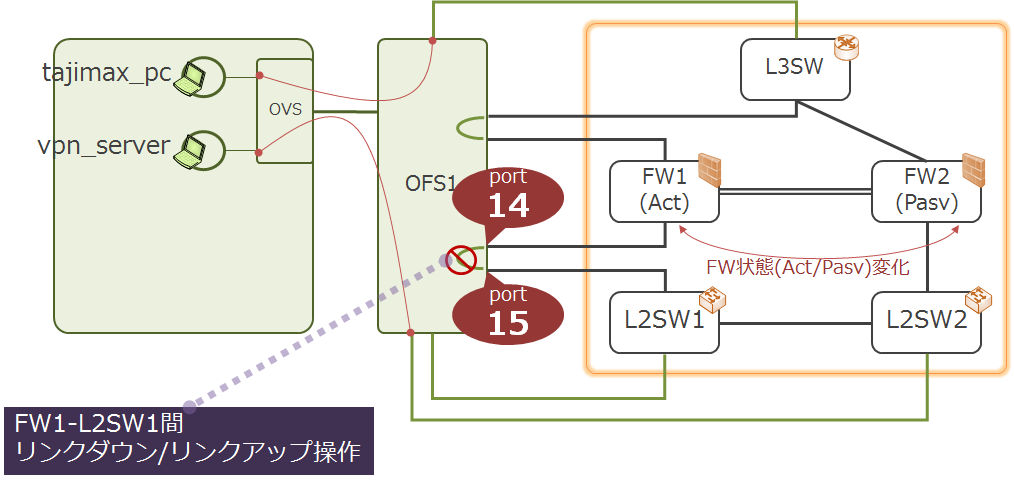
\includegraphics[scale=0.6]{img/poc-env-linkdown.png}
 \caption{PoC環境: NetTesterによるリンクダウン操作}
 \label{fig:poc-env-linkdown}
\end{figure}

\begin{itemize}
 \item 実装 (NAT IPの変更とかデモの話をどこまで含めるか?)
 \item 結果
\end{itemize}

\section{テストシナリオ実装における検討ポイント}

\subsection{Teardown処理}

\begin{itemize}
 \item Target network の状態
       \begin{itemize}
        \item ARP Table のクリア
        \item NAT Table のクリア
        \item Firewall の active/standby (自動復旧にしているのでとくにいれていない)
       \end{itemize}
 \item Netns の /etc 配下のクリア
       \begin{itemize}
        \item 自作echoサーバーで通信開始時に10秒のラグが起きる問題 – NetTester \url{https://3.basecamp.com/3088280/buckets/867009/todos/274457003}
       \end{itemize}
 \item 物理OFSのflow tableのクリア (まだやれてない)
\end{itemize}

\subsection{テストシナリオのサイズ}

シナリオサイズの目安、シナリオ分割の目安 (step3 test つくっているときに
分割するって話になった理由は?)

\subsection{ステップ実装上の工夫}
\begin{itemize}
 \item ニセ○○サーバとステップ実装 – NetTester \url{https://3.basecamp.com/3088280/buckets/867009/documents/216490375}
 \item コマンドをバックグラウンド実行 – NetTester \url{https://3.basecamp.com/3088280/buckets/867009/documents/216399643}
 \item step内でのバックグラウンドコマンド実行 – NetTester \url{https://3.basecamp.com/3088280/buckets/867009/todos/202691188}
 \item factory\_girl で仮想ホストを作る – NetTester \url{https://3.basecamp.com/3088280/buckets/867009/documents/210831650}
\end{itemize}

\section{PoC結果}

結果まとめ

%%% Local Variables:
%%% mode: yatex
%%% TeX-master: "main.tex"
%%% End:
